\documentclass[
	ngerman,
	fontsize=10pt,
	parskip=half,
	titlepage=true,
	DIV=12
]{scrartcl}

\usepackage[utf8]{inputenc}
\usepackage{babel}
\usepackage[T1]	{fontenc}
\usepackage{lmodern}
\usepackage{microtype}
\usepackage{color}
\usepackage{csquotes}

\usepackage{hyperref}


\usepackage{graphicx}
\usepackage{wrapfig}
\usepackage[bf]{caption}
	\captionsetup{format=plain}

\newcommand*{\tabcrlf}{\\ \hline}

\usepackage{amsmath}

\usepackage{minted}
	\usemintedstyle{friendly}

\newcommand*{\inPy}[1]{\mintinline{python3}{#1}}
\newcommand*{\ie}{i.\;e. }
\newcommand*{\eg}{e.\;g. }

\newcommand{\thus}{\ensuremath{\rightarrow}}

	
\begin{document}

\part*{Python Problems 05, Spring 2021}
\section{Characters in a file (2 P)}
Download the file \texttt{praktische\_Physik.txt}\footnote{which you can find online under \url{https://www.familie-ahlers.de/wissenschaftliche_witze/aufgaben_zur_praktischen_physik.html}} from GRIPS and write code that counts the number of characters (with and without line breaks), words and lines in a file. Print your results on screen.

\section{File size with \inPy{tell} and \inPy{seek} (1 P)}
Use the methods \inPy{tell} and \inPy{seek}, to find out the length of a file in bytes.

\section{Total Score (1 P)}
Sebi, Simon und Steve have played a game and written their score for every round into a file \texttt{gameScores.txt} (which you'll find on GRIPS). Write a program that reads the scores and puts the totals for each player on screen.

\section{Integral (I) (1 P)}
\begin{wrapfigure}{r}{.3\linewidth}
	\vspace{-50pt}
	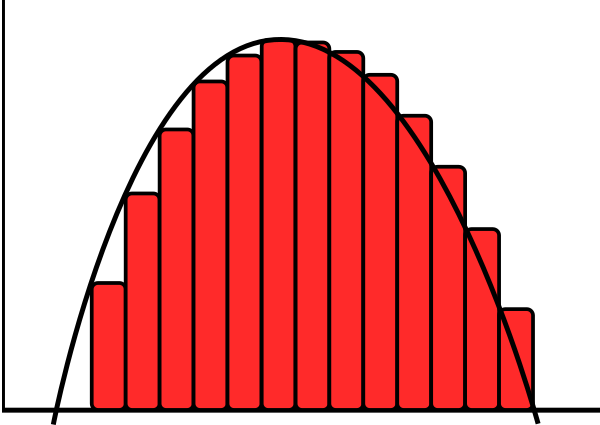
\includegraphics[width=\linewidth]{./integral}
	\caption{Approximation of an integral by area of rectangles.\newline
		Figure by Jonas Süskind}
	\vspace{-50pt}
\end{wrapfigure}
Write a function \texttt{integrate} that approximates the area underneath a graph of a function. The integrand $f$ (\ie the function that gives the graph) should be a parameter to your function \texttt{integrate}. Make it such that your function has the signature:
\mint{python}{def integrate(func, start, stop, N) :}

Use the rectangle approximation:
\begin{itemize}
\item Disect the integration interval into $N$ blocks of equal width
\item For each block, evaluate the function $f$ at the left hand side of your block. This gives the height of the rectangles
\item Find the areas of all $N$ rectangles and sum them up -- this gives you an approximation of the integral
\end{itemize}

You can test your code with the following call:
\mint{python}{print(integrate(math.exp, 0, 1, 10000))}
The output should, approximately, be \texttt{1.718}.


\section{N-Fold Concatenation (2 P)}
Write a function \texttt{concatenateNFold} that computes the value of a function $f$ after n-fold concatenation. That is, the result of 
\texttt{concatenateNFold(f, 3, x)}
should be $f(f(f(x)))$.

\emph{Hint}:\\
Test your code with $f(x) = x + 1$ and $x = 0$. If your code is correct, then the output for \texttt{concatenateNFold(f, N, 0)} should be $N$.



\end{document}
